%%%%%%%%%%%%%%%%%%%%%%%%%%%%%%%%%%%%%%%%%%%%%%%%%%%%%%%%%%%%%%%%%%%%%%
%%                     Modulation
%%%%%%%%%%%%%%%%%%%%%%%%%%%%%%%%%%%%%%%%%%%%%%%%%%%%%%%%%%%%%%%%%%%%%%
%\color{blue}
\subsubsection{Glyph: \glyph{Modulation}}\label{sec:modulation}

A \glyph{modulation} affects the strength, or the probability to exist, of the target relationship. Such a modulation can affect the relationship \textbf{positively or negatively}, or even both ways depending on the conditions. A \glyph{modulation} can also be used when one does not know the precise direction of the effect, for instance if there are conflicting evidence.

\begin{glyphDescription}
 \glyphSboTerm SBO:0000168 ! control.
 \glyphOrigin Any \glyph{entity node} (\sect{ENs}).
 \glyphTarget Any \glyph{relationship} (\sect{relationships}).
 \glyphEndPoint The target extremity of a \glyph{modulation} carries an empty diamond.
 \glyphAux A \glyph{unit of information} carrying the mention \glyph{cis} or \glyph{trans} precises the relationship between the \glyph{entity node} from which the \glyph{modulation} origins and either:
\begin{itemize}
\item the \glyph{entity node} from which the influence targeted by the \glyph{modulation} origins
\item all the relevant \glyph{interactors} of the \glyph{interaction} or the \glyph{non-interaction} targeted by the \glyph{modulation}
\item the \glyph{entity} subjected to the \glyph{assignment} targeted by the \glyph{modulation}
\end{itemize}
 \end{glyphDescription}

\begin{figure}[H]
  \centering
  
\includegraphics[scale = 0.5]{images/modulation}
  \caption{The \ER glyph for \glyph{modulation}.}
  \label{fig:modulation}
\end{figure}
 
% \begin{figure}[H]
%   \centering
%   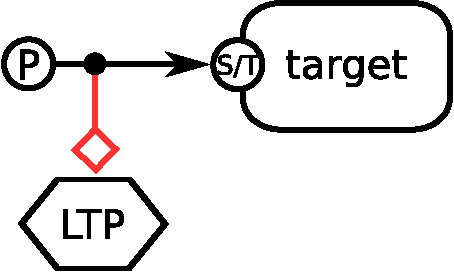
\includegraphics[scale = 0.5]{examples/ex-modulation}
%   \caption{Example of a \glyph{modulation} of the \glyph{phenotype} ``Long Term Potentiation (LTP)'' by the phosphorylation of an \glyph{entity} ``target''. For instance the influence could be positive (stimulation, see \sect{stimulation}) or negative (inhibition, see \sect{inhibition}).}
%   \label{fig:ex-modulation}
% \end{figure}

%\normalcolor

